% 6장 누구에게 달랐나. 이 연구의 뼈대. 0015 · 0019 · 0021 · 0022 · 0023 · 0029
% 이야기 순서로 쓴다 — 서술이 세 번 바뀐 과정을 숨기지 않는다.

\section{누구에게 달랐나}

이 장은 \textbf{결론만 적지 않고 결론에 이른 순서대로} 쓴다. 서술이 세 번 바뀌었고,
바뀐 과정 자체가 이 연구에서 가장 값어치 있는 부분이기 때문이다.

\begin{table}[htbp]
  \centering
  \caption{이질성 서술이 바뀐 과정}
  \label{tab:het-history}
  \begin{tabular}{llp{7.0cm}}
    \toprule
    \textbf{시점} & \textbf{서술} & \textbf{근거} \\
    \midrule
    1주차 & 15억 이하에서 효과가 더 컸다 & 표본을 갈라 따로 추정 \\
    2주차 & 고가 단지에 집중된다 & 삼중차분 ($p=0.0006$) \\
    3주차 & 방향은 맞으나 단단하지 않다 & 적은 클러스터 추론 \\
    3주차 & \textbf{가격이 아니라 면적 기준일 수 있다} &
      경계 민감도 + 면적대 탐색 \\
    3주차 & \textbf{면적 기준이 주된 원인이다} &
      2022 강화 + 2021 위약 \\
    \bottomrule
  \end{tabular}
\end{table}

\textbf{주 결과(지정 직후 $-71 \sim -80\%$)는 한 번도 움직이지 않았다.} 흔들린
것은 이질성의 해석이다.

\subsection{1주차 질문 --- 대출을 고려해야 하지 않나}

1차 발표에서 지도교수가 ``대출 규제를 고려해야 하는 것 아니냐''고 물었다. 근거
없는 지적이 아니었다. 처치군 거래의 \textbf{63.9\%}가 시가 15억원 초과이고 통제
자치구는 0.3$\sim$3.9\%다. 같은 서울 안에서 노출도가 20배 차이난다. 그리고
15억 초과 주담대 금지(2019-12-17)는 토허구역 지정(2020-06-23)보다 \textbf{6개월
앞선다.}

\subsection{대출 규제 25건을 상쇄 10 / 핵심 4 로 가르다}

대출 규제는 토허제와 자료의 성격이 다르다(0015). 토허제는 ``어디가 언제''가
공고에만 있어 공고를 다 모아야 했지만, 대출 규제는 대부분 \textbf{``어디''가
없다} --- 전국 또는 규제지역 일률이다. 그리고 상당수가 금융감독원 행정지도로 나가
관보에 다 남지도 않는다. \textbf{`전수 수집'이라는 접근 자체가 성립하지 않는다.}

그래서 \textbf{증거 등급}을 나눠 2016년 이후 25건을 1차 자료로 확인하고(1차 19건,
시행일 불명 4건), \textbf{처치군과 통제군에 다르게 걸리는가} 하나로 갈랐다.

\begin{table}[htbp]
  \centering
  \caption{대출 규제 25건의 분류}
  \label{tab:loan-class}
  \begin{tabular}{llp{8.0cm}}
    \toprule
    \textbf{분류} & \textbf{건수} & \textbf{뜻} \\
    \midrule
    \textbf{상쇄} & 10 & 서울 전역 동일 적용. 시간 고정효과가 흡수한다 \\
    \textbf{핵심} & 4 & 집값에 걸려 처치군에 집중된다 \\
    나머지 & 11 & 창 밖 · 영향 작음 · 확인 필요 \\
    \bottomrule
  \end{tabular}
\end{table}

\textbf{규제를 다 모을 필요가 없다는 것이 핵심 통찰이다.} 이중차분에서 양쪽에
똑같이 걸리는 규제는 시간 고정효과가 저절로 뺀다. 다르게 걸리는 것만 골라내면 된다.

남는 넷은 2019-12-17 시가 15억 초과 주담대 전면 금지, 2019-12-23 9억 초과분
LTV 40$\to$20\%, 같은 날 9억 초과 차주단위 DSR 40\%, 그리고 2022-12-01 15억 금지
폐지다. \textbf{넷 다 지역이 아니라 집값에 걸린다.}

\textbf{규제가 실제로 물렸는지부터 확인했다.} 문턱 바로 아래와 위($\pm$0.5억)의
거래 수 비를 재면\citep{bestkleven2018} 규제 이전 0.96배, 금지 기간 \textbf{1.60배},
폐지 이후 1.09배다. 분기별로는 금지 직후 2.1배까지 올랐다가 폐지 분기에 0.81로
떨어진다. \textbf{규제가 켜질 때 쏠림이 생기고 꺼지자 사라진다.}

\begin{figure}[htbp]
  \centering
  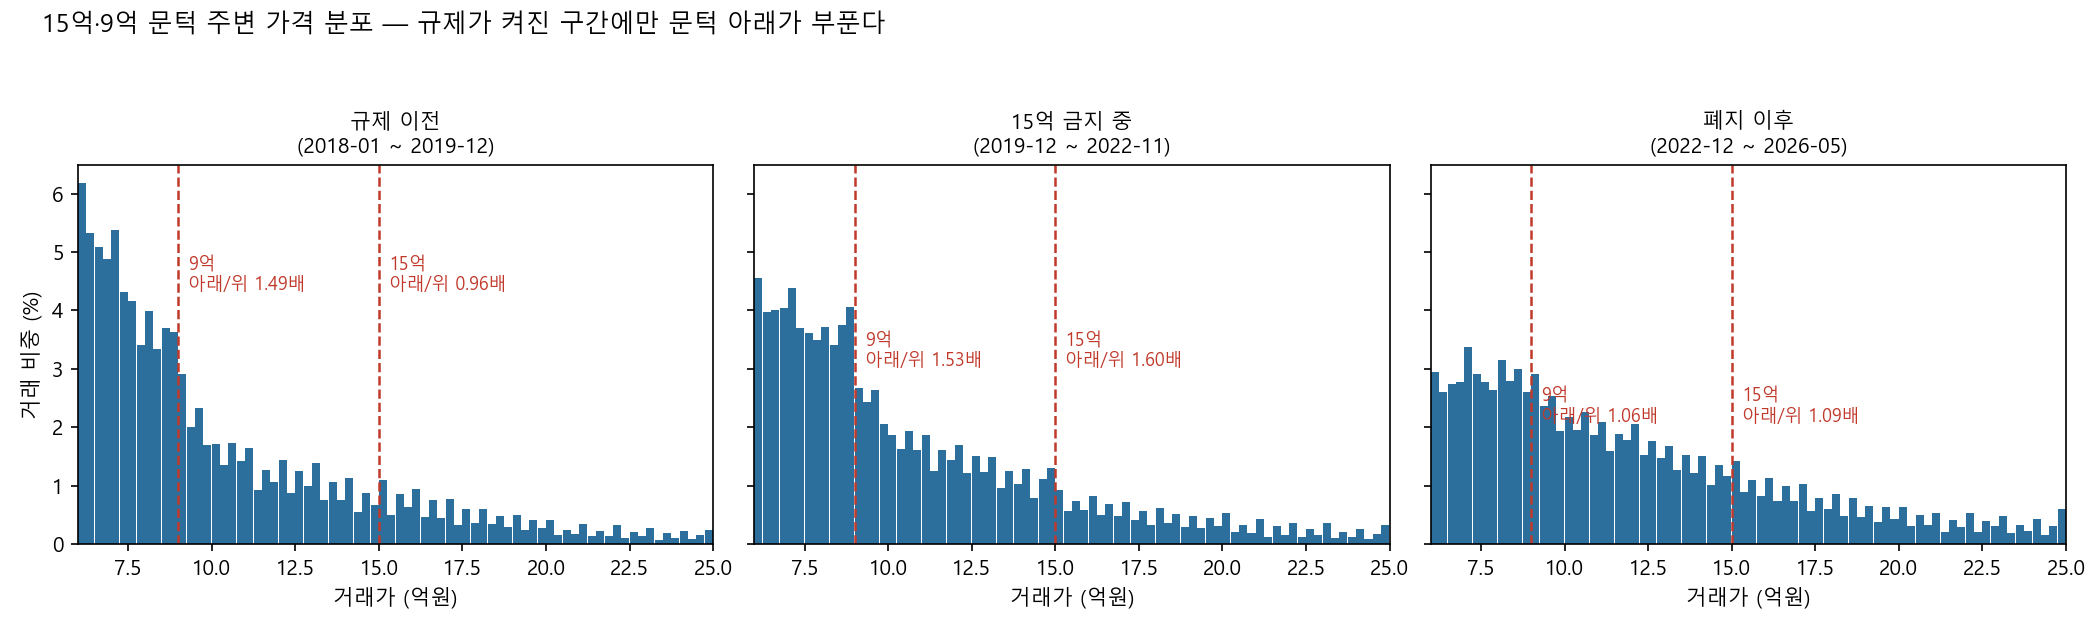
\includegraphics[width=\linewidth]{06c_bunching.png}
  \caption{15억원 문턱의 쏠림. 규제를 따라 켜지고 꺼진다.}
  \label{fig:bunching}
\end{figure}

\textbf{그리고 교란변수가 아님을 셋으로 확인했다.} 첫째, 수준의 불균형은
이중차분에서 문제가 아니다 --- 필요한 것은 추세의 평행이고 수준은 고정효과가
뺀다. 둘째, 상쇄 10건은 시간 고정효과가 먹는다. 셋째, 핵심 4건은 집값에 걸리므로
\textbf{같은 가격대 안에서 비교하면 차분으로 빠진다.} 실제로 고가 통제동이 45\%
줄 때 고가 처치동은 76\% 줄었다. 그리고 12·16 대책을 사전 구간에서 빼든 넣든
$k=0$이 $-73 \sim -74\%$로 바뀌지 않는다(4.5절).

\subsection{삼중차분 --- 고가 단지에 집중된다}

교란이 아니라면 \textbf{이질성 요인}인가. 여기서 두 개념을 구별해야 한다.
교란변수는 처치와 결과에 동시에 영향을 주어 추정치를 \emph{편향}시키고 통제해야
한다. 이질성 요인은 처치 효과의 \emph{크기}를 좌우하므로 \textbf{나눠 봐야 하고
통제하면 안 된다} --- 통제하면 가격 수준 자체를 통제하게 되어 효과의 일부를
빨아들인다(나쁜 통제).

처치군 안에서 15억 초과·이하를 갈라 한 식에 교차항으로 넣었다. \textbf{노출도는
처치 이전에 정해진 값이어야 하므로} 거래 시점 가격이 아니라 12·16 시행 직전 2년의
단지별 중위 거래가를 기준가로 삼았다(전체 거래의 94\%에 기준가가 붙는다).

\begin{table}[htbp]
  \centering
  \caption{가격군별 원자료 --- 법정동 $\times$ 사건월 칸의 평균 거래 건수}
  \label{tab:loan-raw}
  \begin{tabular}{llrrr}
    \toprule
    \textbf{가격군} & \textbf{집단} & \textbf{사전} & \textbf{사후} &
    \textbf{변화} \\
    \midrule
    저가 & 처치 & 7.6 & 3.9 & $-48\%$ \\
    저가 & 통제 & 20.2 & 10.8 & $-47\%$ \\
    \textbf{고가} & \textbf{처치} & \textbf{42.2} & \textbf{10.3} &
      $\mathbf{-76\%}$ \\
    고가 & 통제 & 15.7 & 8.7 & $-45\%$ \\
    \bottomrule
  \end{tabular}
\end{table}

\textbf{저가는 처치와 통제가 똑같이 줄었고 고가만 처치가 더 줄었다.} 삼중차분도
같은 말을 한다 --- 저가 효과 $+5.4\%$($p=0.502$), 차이 $-0.823$($p=0.001$), 고가
효과 $-53.7\%$다.

이것이 2주차의 결론이었다. \textbf{그리고 3주차에 두 번 흔들린다.}

\textbf{먼저 추론이다}(0019). $p=0.0006$은 법정동 27개·처치 4개의 관행 $p$다.
적은 클러스터에 맞는 추론으로 다시 재면 WCR 0.027, 무작위화 등꼬리 0.037,
절댓값 \textbf{0.106}이다. 방향은 원자료가 뒷받침하나 확신의 정도를 낮춘다.

\subsection{그런데 15억에 계단이 없다}

``15억을 골라서 그 결과가 나온 것 아니냐''에 답하려고 경계를 9·12·15·18·20억으로
옮기며 같은 삼중차분을 돌렸다(0021).

% 자동 생성 — scripts/build_tables.py. 손으로 고치지 않는다.
% 출처: output/results/06f_threshold.json : 결과
\begin{table}[htbp]
  \centering
  \caption{고가·저가 경계를 옮기면. 15억에 계단이 없다.}
  \label{tab:threshold}
  \begin{tabular}{lrrrrr}
    \toprule
    \textbf{경계 (억)} & \textbf{저가 (\%)} & \textbf{고가 (\%)} & \textbf{차이 (로그)} & \textbf{WCR $p$} & \textbf{무작위화 $p$} \\
    \midrule
    9 & 52.7 & -44.9 & -1.019 & 0.011 & $<0.001$ \\
    12 & 29.7 & -54.0 & -1.036 & 0.017 & $<0.001$ \\
    15 & 5.4 & -53.7 & -0.823 & 0.032 & 0.037 \\
    18 & -24.7 & -53.6 & -0.484 & 0.026 & 0.189 \\
    20 & -28.4 & -43.7 & -0.240 & 0.426 & 0.450 \\
    \bottomrule
  \end{tabular}

  \begin{minipage}{\linewidth}\footnotesize
  \textit{주.} 경계를 어디에 두든 고가 효과는 $-44 \sim -54\%$ 로 평평하고, 저가 효과는 경계를 따라 매끈하게 움직인다.
  \end{minipage}
\end{table}


\begin{figure}[htbp]
  \centering
  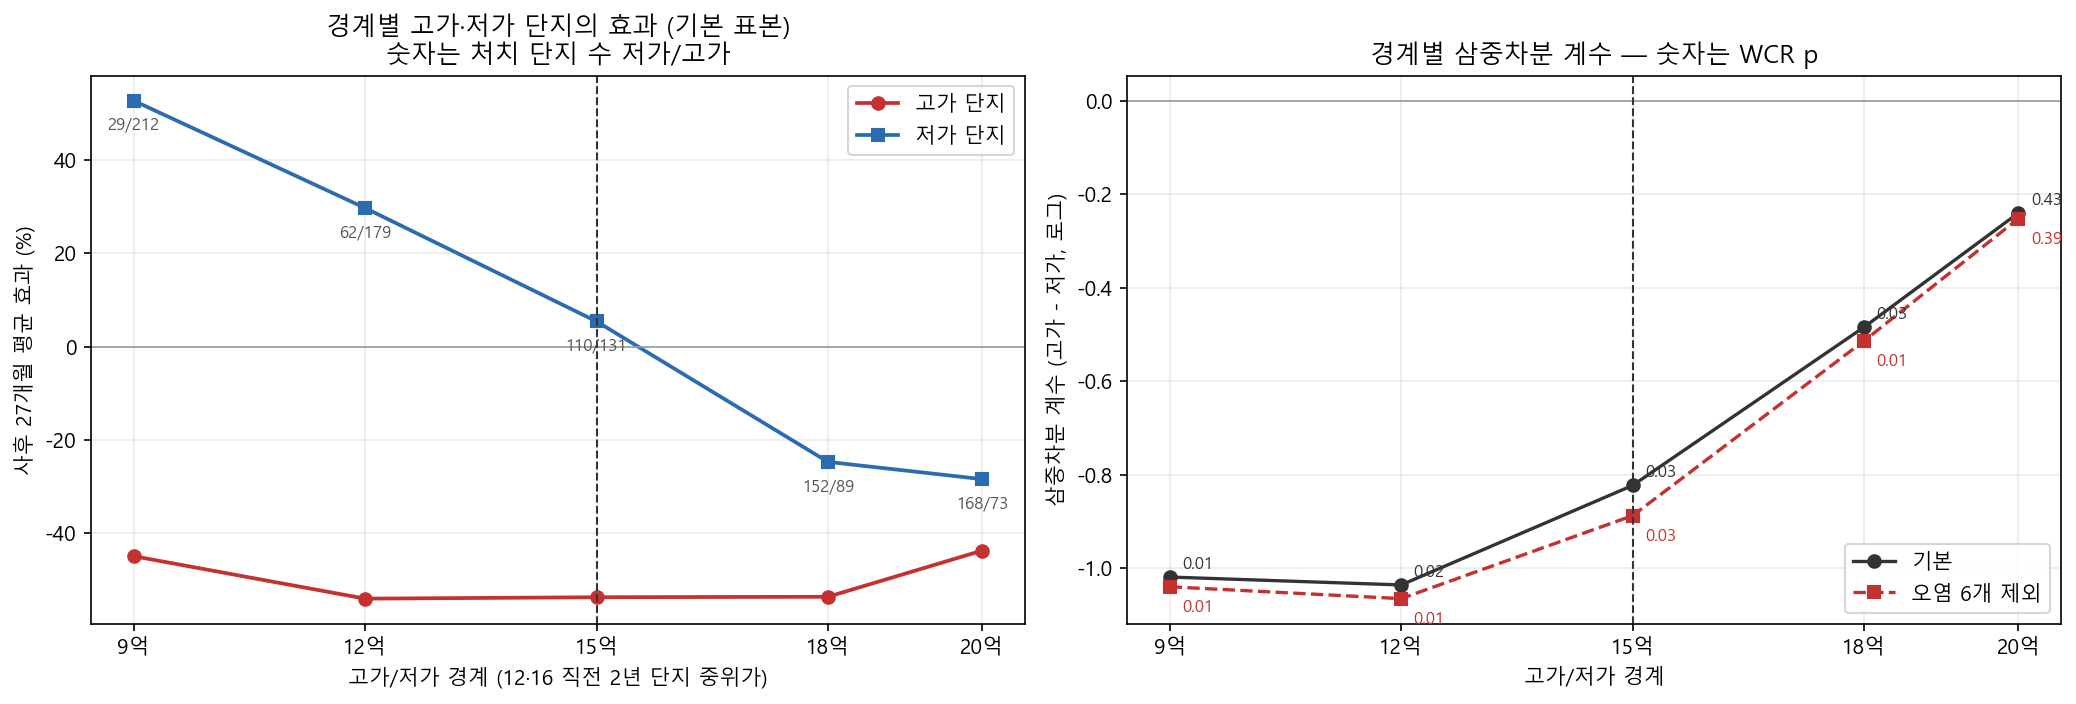
\includegraphics[width=\linewidth]{06f_threshold.png}
  \caption{고가·저가 경계를 9$\sim$20억으로 옮길 때. 15억에 계단이 없다.}
  \label{fig:threshold}
\end{figure}

읽을 것이 셋이다.

\textbf{첫째, 고가 효과는 어느 경계에서나 $-44 \sim -54\%$다.} 15억을 골라서 나온
결과가 아니다. 이 점에서는 2주차 결론이 보강된다.

\textbf{둘째, 저가 효과는 경계를 따라 미끄러진다.} $+52.7\%$에서 $-28.4\%$까지
부드럽게 내려간다. 경계를 올리면 12억·15억짜리 단지가 `저가'로 넘어오는데 그
단지들도 크게 줄었기 때문이다.

\textbf{셋째 --- 그리고 결정적으로 --- 15억에 계단이 없다.} 대출이 이질성을
만들었다면 15억 초과는 대출이 이미 막혀 있었고 15억 이하는 아니었으므로 효과가
15억을 사이에 두고 \textbf{뚝 끊겨야} 한다. 자료는 그렇지 않다. 고가 효과가
12·15·18억에서 $-54.0$, $-53.7$, $-53.6\%$로 평평하다. \textbf{15억은 자료 안에서
특별한 자리가 아니다.}

\subsection{`저가'는 사실상 `소형'이었다}

경계를 낮출수록 `저가'가 무엇과 겹치는지 보았다. \textbf{9억 이하 처치 단지 거래의
전용면적 중위값이 36.4\,m$^2$}다. 9억 초과는 84.8\,m$^2$다.

그리고 2020년 6월 지정의 허가 대상은 \textbf{주거지역 대지 18\,m$^2$ 초과}였다.
대지지분이 작은 소형은 구역 안에 있어도 \textbf{허가 없이 살 수 있었다.}

전용면적대별로 원자료를 보면 모양이 분명하다.

\begin{table}[htbp]
  \centering
  \caption{전용면적대별 거래 변화 (사전 24개월 대비 사후 27개월 월평균)}
  \label{tab:area-raw}
  \begin{tabular}{lrrrr}
    \toprule
    \textbf{전용면적} & \textbf{처치 사전 월평균} & \textbf{처치 변화} &
    \textbf{통제 변화} & \textbf{차이} \\
    \midrule
    \textbf{40\,m$^2$ 미만} & 10.0 & $\mathbf{+7.3\%}$ & $-3.6\%$ &
      $\mathbf{+10.9}$\,\%p \\
    40$\sim$60 & 24.3 & $-73.1\%$ & $-51.2\%$ & $-21.9$\,\%p \\
    60$\sim$85 & 96.2 & $-76.8\%$ & $-50.6\%$ & $-26.2$\,\%p \\
    85$\sim$135 & 42.5 & $-76.3\%$ & $-50.7\%$ & $-25.6$\,\%p \\
    135 이상 & 25.5 & $-65.8\%$ & $-41.4\%$ & $-24.5$\,\%p \\
    \bottomrule
  \end{tabular}
\end{table}

\textbf{40\,m$^2$ 미만만 줄지 않았고, 40\,m$^2$ 이상은 크기와 상관없이
$-22 \sim -26$\,\%p로 거의 같다.} 가장 비싼 135\,m$^2$ 이상과 가장 싼
40$\sim$60\,m$^2$가 같은 폭이다.

\textbf{이 모양은 대출 이야기보다 면적 면제 이야기에 맞는다.} 대출이 원인이면
40\,m$^2$ 이상 \emph{안에서도} 비쌀수록 더 줄어야 하는데 그렇지 않다. 면제가
원인이면 면제된 소형만 빠지고 나머지는 같게 줄어야 하는데 그렇다.

\subsection{2022년 기준 강화가 두 가설을 갈랐다}

여기까지는 탐색이다. 두 가설이 \textbf{반대 방향을 예측하는 사건}이 자료 안에
있었다(0022).

\begin{table}[htbp]
  \centering
  \caption{두 가설이 예측하는 것}
  \label{tab:two-hyp}
  \begin{tabular}{lll}
    \toprule
    \textbf{가설} & \textbf{규제가 다르게 물린 축} & \textbf{예측} \\
    \midrule
    대출 & 가격 & 15억을 사이에 두고 효과가 끊긴다 \\
    \textbf{면제} & \textbf{크기} &
      소형만 빠지고, 면제가 사라지면 소형도 줄어든다 \\
    \bottomrule
  \end{tabular}
\end{table}

\textbf{2022년 6월 23일에 허가 기준이 대지 18\,m$^2$에서 6\,m$^2$로 강화됐다}
(서울특별시공고 제2022-1795호 원문에서 확인). 이날 처치 4개 동의 \textbf{소형만}
새로 허가 대상이 된다. 대형은 이미 대상이었으므로 바뀌는 것이 없다.
\textbf{대출 가설은 이 날짜에 아무것도 예측하지 않는다.}

% 자동 생성 — scripts/build_tables.py. 손으로 고치지 않는다.
% 출처: output/results/06g_area_exemption.json : 나_2022_기준강화
\begin{table}[htbp]
  \centering
  \caption{2022-06-23 허가 면적 기준 강화(대지 18 $\to$ 6\,m$^2$). 소형만 줄었다.}
  \label{tab:area-2022}
  \begin{tabular}{lrrrrr}
    \toprule
    \textbf{소형 경계 (m$^2$)} & \textbf{처치 소형 거래} & \textbf{소형 (\%)} & \textbf{대형 (\%)} & \textbf{WCR $p$} & \textbf{무작위화 $p$} \\
    \midrule
    30 & 62 & -26.2 & 17.1 & 0.082 & 0.111 \\
    40 & 130 & -33.2 & 21.7 & 0.021 & 0.016 \\
    50 & 141 & -30.9 & 21.0 & 0.022 & 0.055 \\
    60 & 212 & -19.8 & 12.1 & 0.123 & 0.108 \\
    \bottomrule
  \end{tabular}

  \begin{minipage}{\linewidth}\footnotesize
  \textit{주.} 그날 처치동 소형만 새로 허가 대상이 된다. 대출 가설은 이 날짜에 아무것도 예측하지 않는다.
  \end{minipage}
\end{table}


\begin{figure}[htbp]
  \centering
  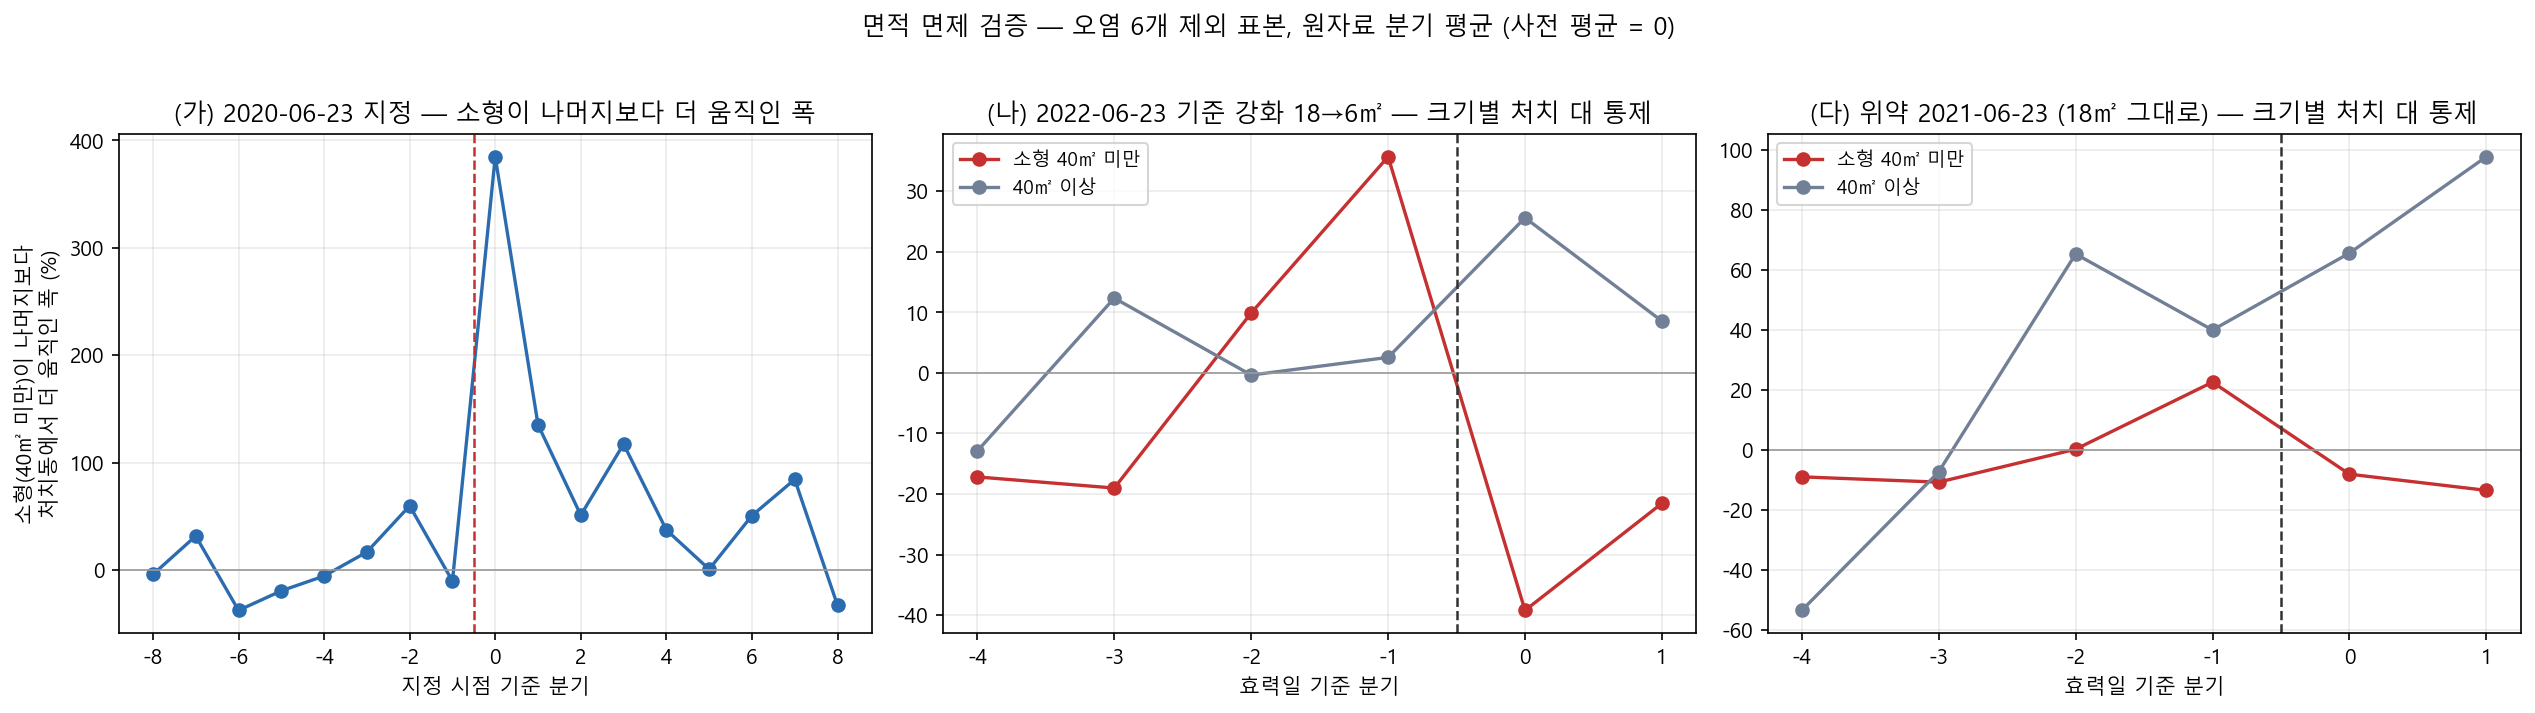
\includegraphics[width=\linewidth]{06g_area_exemption.png}
  \caption{면적 면제 검증. 가운데가 2022년 기준 강화, 오른쪽이 2021년 위약.
           빨간 선이 소형(40\,m$^2$ 미만)이다.}
  \label{fig:area-exemption}
\end{figure}

\textbf{소형만 줄었다.} 40\,m$^2$ 경계에서 $-33.2\%$(WCR 0.023, 무작위화 0.001)이고
\textbf{대형은 오히려 올라간다}($+21.7\%$, 0.236).

\textbf{첫 설계는 위약에서 실패했음을 밝혀 둔다.} 처음에는 처치동 소형과 처치동
대형을 견주는 삼중차분으로 했는데, 2021년 위약이 $-0.715$로 진짜($-0.600$)만큼
크게 나왔다. 원인은 비교 기준이었다 --- 2021년 위약의 사전 구간은 2020년 지정 직후
1년이라 처치동 대형이 폭락해 있던 때이고, 사후에 대형이 회복하니 ``소형이
상대적으로 줄었다''로 보였다. \textbf{대형을 비교 기준에서 빼고 같은 크기끼리
처치동 대 통제동으로 다시 쟀다.}

\subsection{위약 --- 2021년 재지정}

2021년 6월 23일 재지정은 같은 계절, 같은 행정 절차였지만 \textbf{면적 기준을
18\,m$^2$ 그대로 두었다.} 소형에게 바뀐 것이 없으므로 효과가 0이어야 한다.

% 자동 생성 — scripts/build_tables.py. 손으로 고치지 않는다.
% 출처: output/results/06g_area_exemption.json : 다_2021_위약
\begin{table}[htbp]
  \centering
  \caption{위약 --- 2021-06-23 재지정. 면적 기준을 그대로 두었다.}
  \label{tab:area-2021}
  \begin{tabular}{lrrrr}
    \toprule
    \textbf{소형 경계 (m$^2$)} & \textbf{소형 (\%)} & \textbf{대형 (\%)} & \textbf{WCR $p$} & \textbf{무작위화 $p$} \\
    \midrule
    30 & -14.5 & 72.0 & 0.009 & 0.009 \\
    40 & -8.1 & 87.8 & 0.016 & 0.011 \\
    50 & 6.2 & 84.2 & 0.025 & 0.038 \\
    60 & 20.7 & 83.2 & 0.034 & 0.047 \\
    \bottomrule
  \end{tabular}

  \begin{minipage}{\linewidth}\footnotesize
  \textit{주.} 같은 계절, 같은 행정 절차인데 소형에 바뀐 것이 없다. 0 이어야 한다.
  \end{minipage}
\end{table}


\textbf{소형은 규칙이 바뀐 해에만 줄었다.} 2021년에는 $-8.1\%$($p=0.61$)로 0과
구분되지 않고, 2022년에는 $-33.2\%$($p=0.023$)다. 직전 분기를 빼도 $-27.4\%$가
남고, 사전 24개월로 늘려도 $-32.1\%$다. 소형 경계를 옮겨도 30\,m$^2$ $-26\%$,
40 $-33\%$, 50 $-31\%$, 60 $-20\%$로 유지된다(60에서 약해지는 것은 대지 18\,m$^2$를
넘는 단지가 섞여 들어오기 때문으로 읽는다).

\textbf{소형을 빼면 15억 가격 차이가 유의하지 않아진다.} 전체 표본에서 차이가
$-0.823$(무작위화 0.037)인데 40\,m$^2$ 이상만 남기면 $-0.669$(무작위화
\textbf{0.098})가 된다. \textbf{가격 차이의 상당 부분이 소형이었다.}

\subsection{사전 등록한 예측이 맞았다}

4.7절에 적어 둔 예측을 확인할 차례다. 2025년 2월 13일 A그룹이 대부분 해제됐다가
\textbf{39일 만인 3월 24일} 강남3구·용산 전체 아파트로 재지정됐다. 이번 지정의
허가 기준은 \textbf{6\,m$^2$}이므로 소형 면제가 거의 없다.

% 자동 생성 — scripts/build_tables.py. 손으로 고치지 않는다.
% 출처: output/results/09_release_2025.json : 크기_삼중차분
\begin{table}[htbp]
  \centering
  \caption{면적 기준이 바뀌자 효과의 모양이 바뀌었다. 2022년에 적어 둔 예측이 2025년 자료에서 확인됐다.}
  \label{tab:size-ddd}
  \begin{tabular}{lrrrrr}
    \toprule
    \textbf{사건} & \textbf{허가 대상} & \textbf{대형 (\%)} & \textbf{소형 (\%)} & \textbf{차이 (로그)} & \textbf{$p$} \\
    \midrule
    2020-06-23 지정 & 대지 18㎡ 초과 & -95.0 & 125.7 & 3.818 & $<0.001$ \\
    2025-03-24 재지정 & 대지 6㎡ 초과 & -89.4 & -71.5 & 0.987 & 0.388 \\
    \bottomrule
  \end{tabular}

  \begin{minipage}{\linewidth}\footnotesize
  \textit{주.} 2020년 지정은 대지 18\,m$^2$ 초과만 허가 대상이라 소형이 면제됐고, 2025년 재지정은 6\,m$^2$ 라 면제가 거의 없다.
  \end{minipage}
\end{table}


\begin{figure}[htbp]
  \centering
  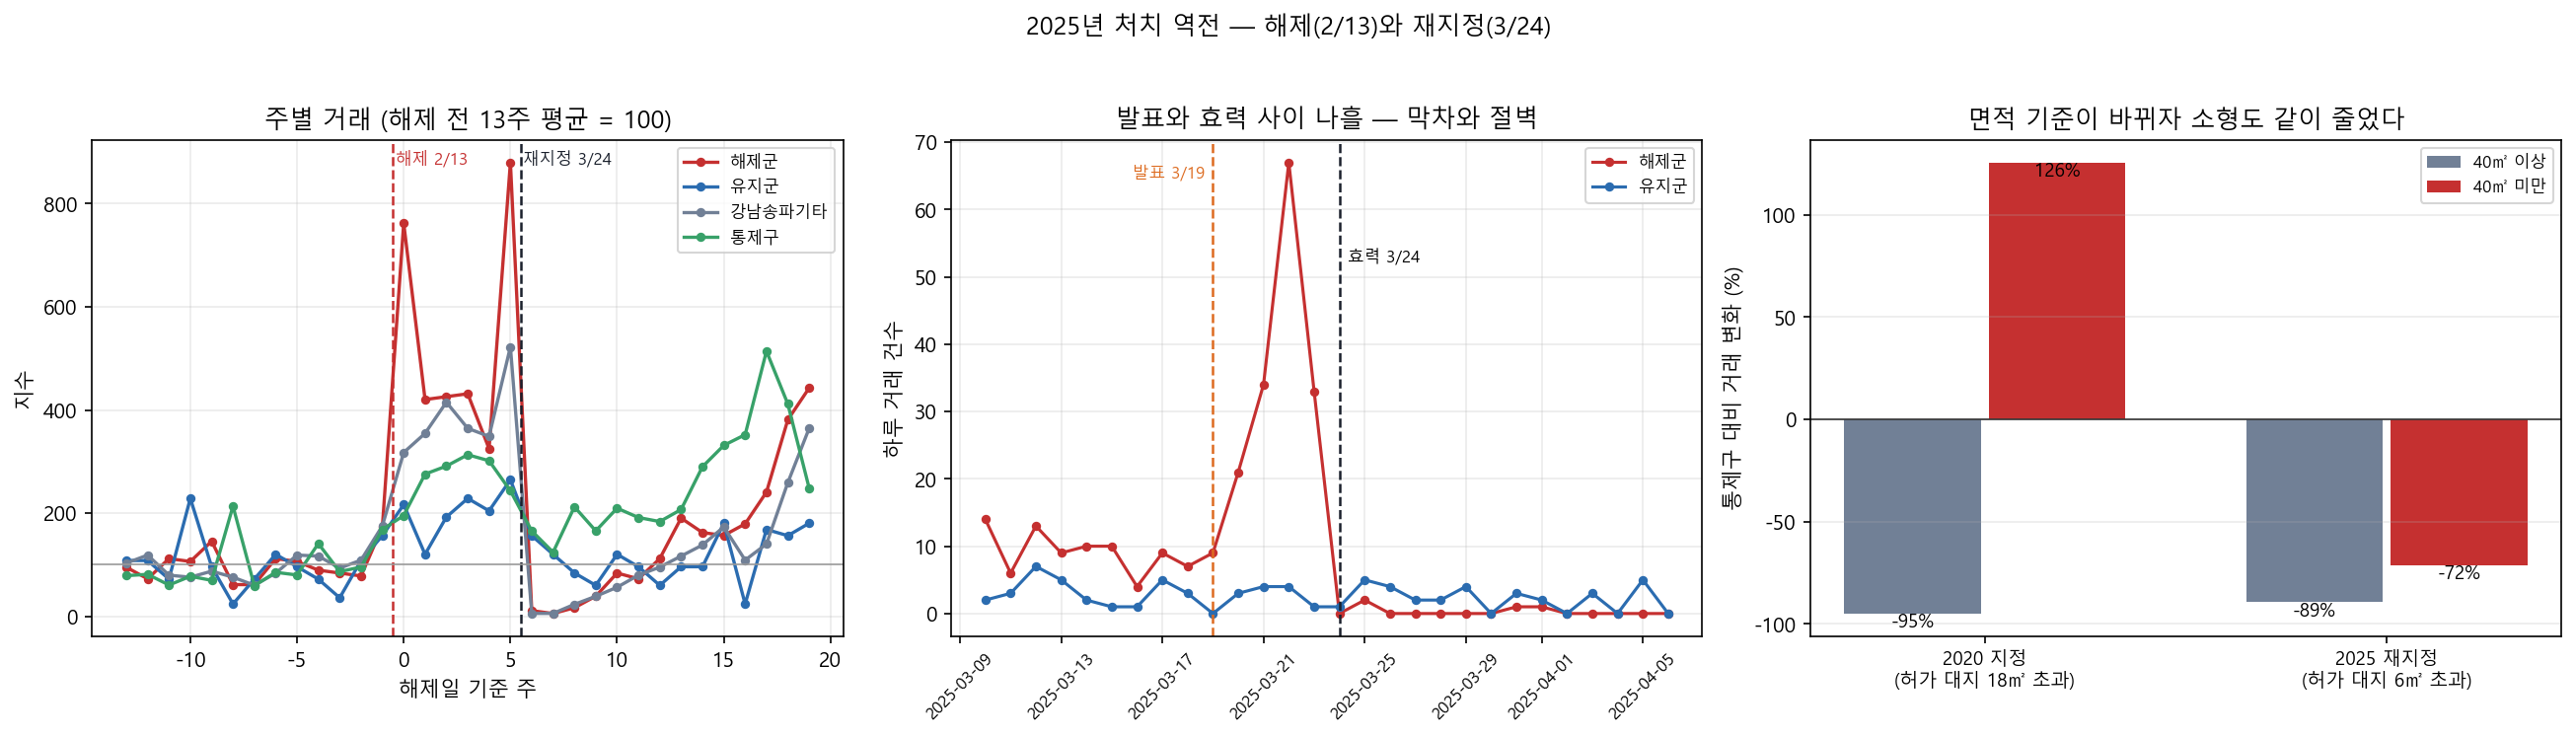
\includegraphics[width=\linewidth]{09_release_2025.png}
  \caption{2025년 처치 역전. 왼쪽 주별 거래, 가운데 발표와 효력 사이 나흘의
           막차와 절벽, 오른쪽 면적 기준이 바뀌자 소형도 줄었다.}
  \label{fig:release-2025}
\end{figure}

\textbf{예측이 맞았다.} 2020년에는 대형 $-95.0\%$ 대 소형 $+125.7\%$로 부호가
반대였는데, 2025년에는 대형 $-89.4\%$ 대 소형 $-71.5\%$로 \textbf{같은 방향}이다.
두 집단의 차이가 2020년 $+3.818$에서 2025년 $+0.987$로 줄었다.

재지정 직후 5주 거래량은 유지군 대비 $-78.9\%$이고(정상 13주 기저), 해제창을
기저로 하면 $-92.3\%$다. 12주로 늘리면 통제군에 따라 $-14\%$와 $-60\%$로 갈리므로
\textbf{지속 기간은 여기서도 말하지 않는다.}

그림 가운데 패널이 덤으로 나온 발견이다. 공고(3월 19일)와 효력(3월 24일) 사이
\textbf{나흘} 동안 하루 거래가 평소 5$\sim$10건에서 \textbf{66건}까지 튀었다가
효력일 다음 날부터 0 근처로 떨어진다. 주간으로 보면 30$\to$155$\to$2건이다.
\textbf{막차 수요가 하루 단위 자료에서만 보인다.} 그리고 그 막차 계약이 나중에
무더기로 취소된 것도 아니다 --- 2020년 막차 구간의 취소율이 3.78\%로 직전 한 달
4.85\%보다 오히려 낮다(9.7절).

\subsection{대출의 몫 --- 작거나 가릴 수 없다}

면적 기준이 주된 원인이라는 결론이 \textbf{대출의 몫이 0이라는 뜻은 아니다.}
소형을 뺀 뒤에도 15억 경계의 차이가 점추정으로 $-0.669$ 남는다. 무작위화로는
유의하지 않다(0.098).

대출 가설을 한 번 더 걸어 보려고 \textbf{15억 금지의 폐지}(2022-12-01)를 사건으로
삼았다(0029). 걸 때 줄었다면 풀 때 돌아와야 한다. \textbf{착수 전에 교란 셋을
적어 두었고 셋 다 현실로 나타났다} --- 그날 9억 꺾임도 함께 풀렸고, 한 달 뒤
2023-01-03 대책이 규제지역을 대거 해제했으며, 2022년 말은 금리 급등기였다.

\begin{table}[htbp]
  \centering
  \caption{금지와 폐지의 거울상 (고가 단지 거래, 저가 대비)}
  \label{tab:mirror}
  \begin{tabular}{lrrr}
    \toprule
    \textbf{사건} & \textbf{$\pm$1개월} & \textbf{$\pm$3개월} &
    \textbf{$\pm$12개월} \\
    \midrule
    2019-12-17 금지 & $-32.2\%$ (0.001) & $-50.7\%$ ($<0.001$) &
      $-33.5\%$ ($<0.001$) \\
    2022-12-01 폐지 & $+21.3\%$ (\textbf{0.380}) & $+81.1\%$ ($<0.001$) &
      $+67.7\%$ ($<0.001$) \\
    \bottomrule
  \end{tabular}
\end{table}

부호가 반대이고 위약도 깨끗하다(2020-12-01 $+0.6\%$, 2021-12-01 $-9.1\%$,
2023-12-01 $+5.1\%$). \textbf{그러나 1·3 대책 이전의 깨끗한 창($\pm$1개월)에서는
유의하지 않다.} 그리고 문턱을 옮기면 폐지 효과가 9억 $+123.9\%$에서 20억
$+69.5\%$로 매끈하게 기울며 \textbf{15억에 아무 일도 일어나지 않는다.}

\begin{figure}[htbp]
  \centering
  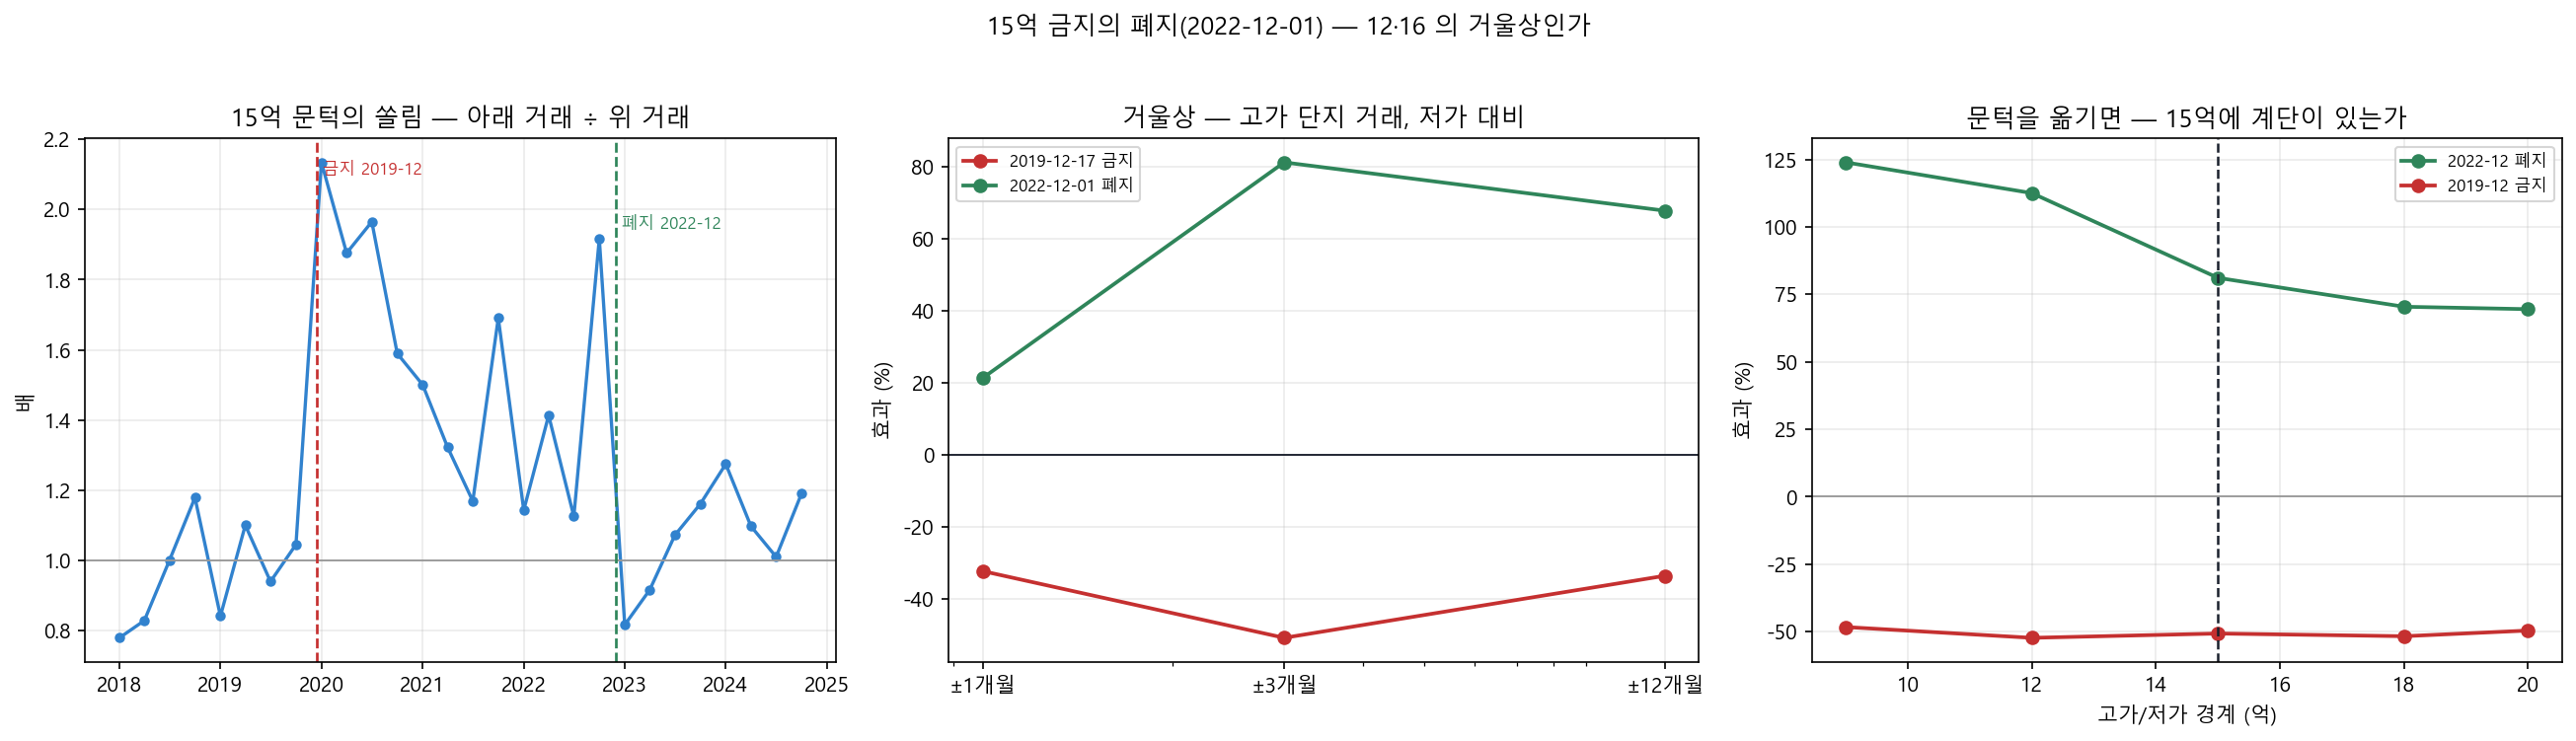
\includegraphics[width=\linewidth]{06e_loan_repeal.png}
  \caption[15억 금지(2019-12)와 그 폐지(2022-12-01) --- 15억에 계단이 없다]{%
    15억 금지(2019-12)와 그 폐지(2022-12-01). \textbf{오른쪽 판이 이
    절의 요지다} --- 가로축을 고가/저가 경계로 삼아 문턱을 9억에서 20억까지
    옮겨도 두 선 모두 \textbf{15억(점선)에서 꺾이지 않는다}. 규제가 15억에
    걸려 있는데 효과가 15억에서 계단을 만들지 않는다면, 그 효과를 대출 규제의
    몫으로 돌릴 수 없다(0021 · 0029). 가운데 판은 금지와 폐지의 부호가 반대라는
    것을, 왼쪽 판은 문턱 아래위 거래 비율이 금지 시점에 2.1배까지 치솟았다가
    폐지 시점에 되돌아오는 것을 보여 준다.}
  \label{fig:loan-repeal}
\end{figure}

\textbf{``폐지 덕에 고가 거래가 돌아왔다''고 쓰지 않는다.} 돌아온 것은 사실이지만
금리 정점 통과와 1·3 대책에서 그 몫을 가를 수 없다. 이 작업의 수확은 오히려
\textbf{``15억에 계단이 없다''를 서울 전역·다른 사건·다른 창에서 재확인}한 것이다.
6.4절은 강남·송파 표본 하나였다.

\subsection{이 장의 결론}

\begin{quote}
대출 규제는 \textbf{교란변수가 아니다}. 토지거래허가제의 효과는 단지마다
달랐는데, 그 차이는 대출 규제보다 \textbf{허가 대상의 면적 기준}으로 더 잘
설명된다. 2020년에는 대지 18\,m$^2$ 이하 소형이 허가 대상에서 빠져 거래가 줄지
않았고, 2022년 기준이 6\,m$^2$로 강화되자 그 소형의 거래가 약 3분의 1 줄었다.
\textbf{대출의 몫은 작거나 가릴 수 없다.}
\end{quote}

근거는 셋이다. 2020년 지정 때 소형은 줄지 않았고, 2022년 기준이 강화되자
\emph{그때} 소형이 줄었으며, 기준을 바꾸지 않은 2021년 재지정에서는 소형이
움직이지 않았다. \textbf{대출 가설은 뒤의 둘을 설명하지 못한다.}
